\documentclass[journal,onecolumn]{IEEEtran}

% * CITATION PACKAGES *
\usepackage{cite}

% * GRAPHICS RELATED PACKAGES *
\usepackage{graphicx}
\graphicspath{{./}{../}{./Week9 work/}{./output_final/}}
\DeclareGraphicsExtensions{.pdf,.jpeg,.jpg,.png}

% * MATH PACKAGES *
\usepackage{amsmath}
\usepackage{amssymb}
\usepackage{amsfonts}
\usepackage{bm}

% * ALIGNMENT PACKAGES *
\usepackage{array}

% * PDF, URL AND HYPERLINK PACKAGES *
\usepackage{url}
\usepackage{booktabs}
\usepackage{microtype}
\usepackage[hidelinks]{hyperref}
\usepackage{float}

% Correct bad hyphenation here
\hyphenation{op-tical net-works semi-conduc-tor}

\begin{document}

% Paper title
\title{Semantic-Aware Integrated Sensing and Communication (ISAC) Networks with Power-Domain NOMA and 3D Elevation-Dependent Path Loss under Uncertain Eavesdropper Locations}

% Author names and affiliations
\author{
Dr. Sunandita Debnath, Dr. Gaurav Kr. Pandey,
Nikhil~Gadige,
Anuj~Saha,
Divyanshu~Ghosh,
Mohli~Thapa%
\thanks{N. Gadige, A. Saha, D. Ghosh, and M. Thapa are with the Department of Computer Science and Engineering, Indian Institute of Information Technology Vadodara.}%
\thanks{E-mails: 202351037@iiitvadodara.ac.in, 202351010@iiitvadodara.ac.in, 202351036@iiitvadodara.ac.in, 202351084@iiitvadodara.ac.in.}
}

% Make the title area
\maketitle

\begin{abstract}
Integrated Sensing and Communication (ISAC) has emerged as a foundational technology for 6G wireless networks to unify spectrum usage, hardware infrastructure, and computing resources. However, simultaneous security vulnerabilities and severe propagation blockages in Air-to-Ground (A2G) channels present major operational bottlenecks. In this report, we present the comprehensive system design and optimization framework for a Semantic-Aware ISAC Network assisted by an aerial Reconfigurable Intelligent Surface (RIS) mounted on a UAV ($R$) and a dedicated cooperative UAV Jammer ($J$). To optimize spectral efficiency, we incorporate Power-Domain Non-Orthogonal Multiple Access (PD-NOMA) to serve a near legitimate user (Target $T$) and a distant mobile user ($U$) over the same time-frequency resource block. Crucially, all legitimate and adversarial communication links are evaluated under semantic-aware metrics via pre-trained DeepSC models, shifting the paradigm from error-free bit recovery to meaning preservation ($M=10, K=15$). The network operates in the presence of $K_e = 3$ terrestrial eavesdroppers ($E_1, E_2, E_3$) whose physical coordinates are imperfectly known (bounded location uncertainty $\Delta Q_e = 15.0\text{ m}$). The UAV Jammer performs monostatic and bistatic radar target tracking while projecting directional artificial noise with spatial null-space suppression ($\eta_{\text{ns}} = 10^{-4}$) at legitimate receivers. We formulate the multi-stage digital and analog beamforming, worst-case wiretap rate expressions under Selection Combining (SC), and the joint multi-objective optimization problem combining Average System Secrecy Ratio (ASSR) and detection probability ($P_d$) under Cram\'{e}r-Rao Bound (CRB) constraints. Finally, we implement and benchmark five reinforcement learning paradigms: Random Walk, Single-Agent TD3PG (SATD3PG), Single-Agent SAC (SASAC), Multi-Agent TD3PG (MATD3PG), and Multi-Agent PPO (MAPPO).
\end{abstract}

\begin{IEEEkeywords}
Integrated Sensing and Communication (ISAC), Semantic Communications, DeepSC, Power-Domain NOMA, Reconfigurable Intelligent Surface (RIS), Location Uncertainty, Null-Space Beamforming, Selection Combining, Deep Reinforcement Learning.
\end{IEEEkeywords}

\IEEEpeerreviewmaketitle

\section{Introduction}
Future 6G wireless systems are envisioned to integrate high-precision radar sensing and artificial intelligence into native communication infrastructures. Integrated Sensing and Communication (ISAC) allows wireless platforms to simultaneously transmit data and extract environmental radar parameters (such as target range, velocity, and angle estimation) using shared spectrum and hardware.

To mitigate urban blockages and severe free-space attenuation in Air-to-Ground (A2G) channels, Reconfigurable Intelligent Surfaces (RIS) deployed on Unmanned Aerial Vehicles (UAVs) ($R$) offer reconfigurable Line-of-Sight (LoS) links between terrestrial Base Stations (BS) $B$ and mobile users. By dynamically adjusting the reflection phase shifts of passive meta-elements, aerial RIS platforms significantly enhance both legitimate signal power and physical layer security.

Concurrently, semantic communications depart from traditional bit-level error minimization by extracting and transmitting only task-relevant semantic features through deep learning encoders (e.g., DeepSC). Semantic representations achieve high compression efficiency, robustness against severe channel fading, and intrinsic confidentiality: an eavesdropper lacking the shared semantic background knowledge cannot reconstruct the source text or intended meaning even when channel symbols are intercepted.

To ensure robust physical layer security against covert eavesdropping, legitimate transceivers cannot assume perfect channel state information (CSI) or exact eavesdropper locations. Instead, terrestrial eavesdroppers are modeled with bounded location uncertainty:
\begin{equation}
    \mathbf{p}_{E_e} = \widetilde{\mathbf{p}}_{E_e} + \Delta\mathbf{p}_{E_e}, \quad \|\Delta\mathbf{p}_{E_e}\|_2 \le \Delta Q_e,
\end{equation}
where $\widetilde{\mathbf{p}}_{E_e}$ is the estimated coordinate and $\Delta Q_e = 15.0\text{ m}$ is the maximum uncertainty radius. We formulate worst-case secrecy capacity under this uncertainty sphere.

\begin{figure}[H]
    \centering
    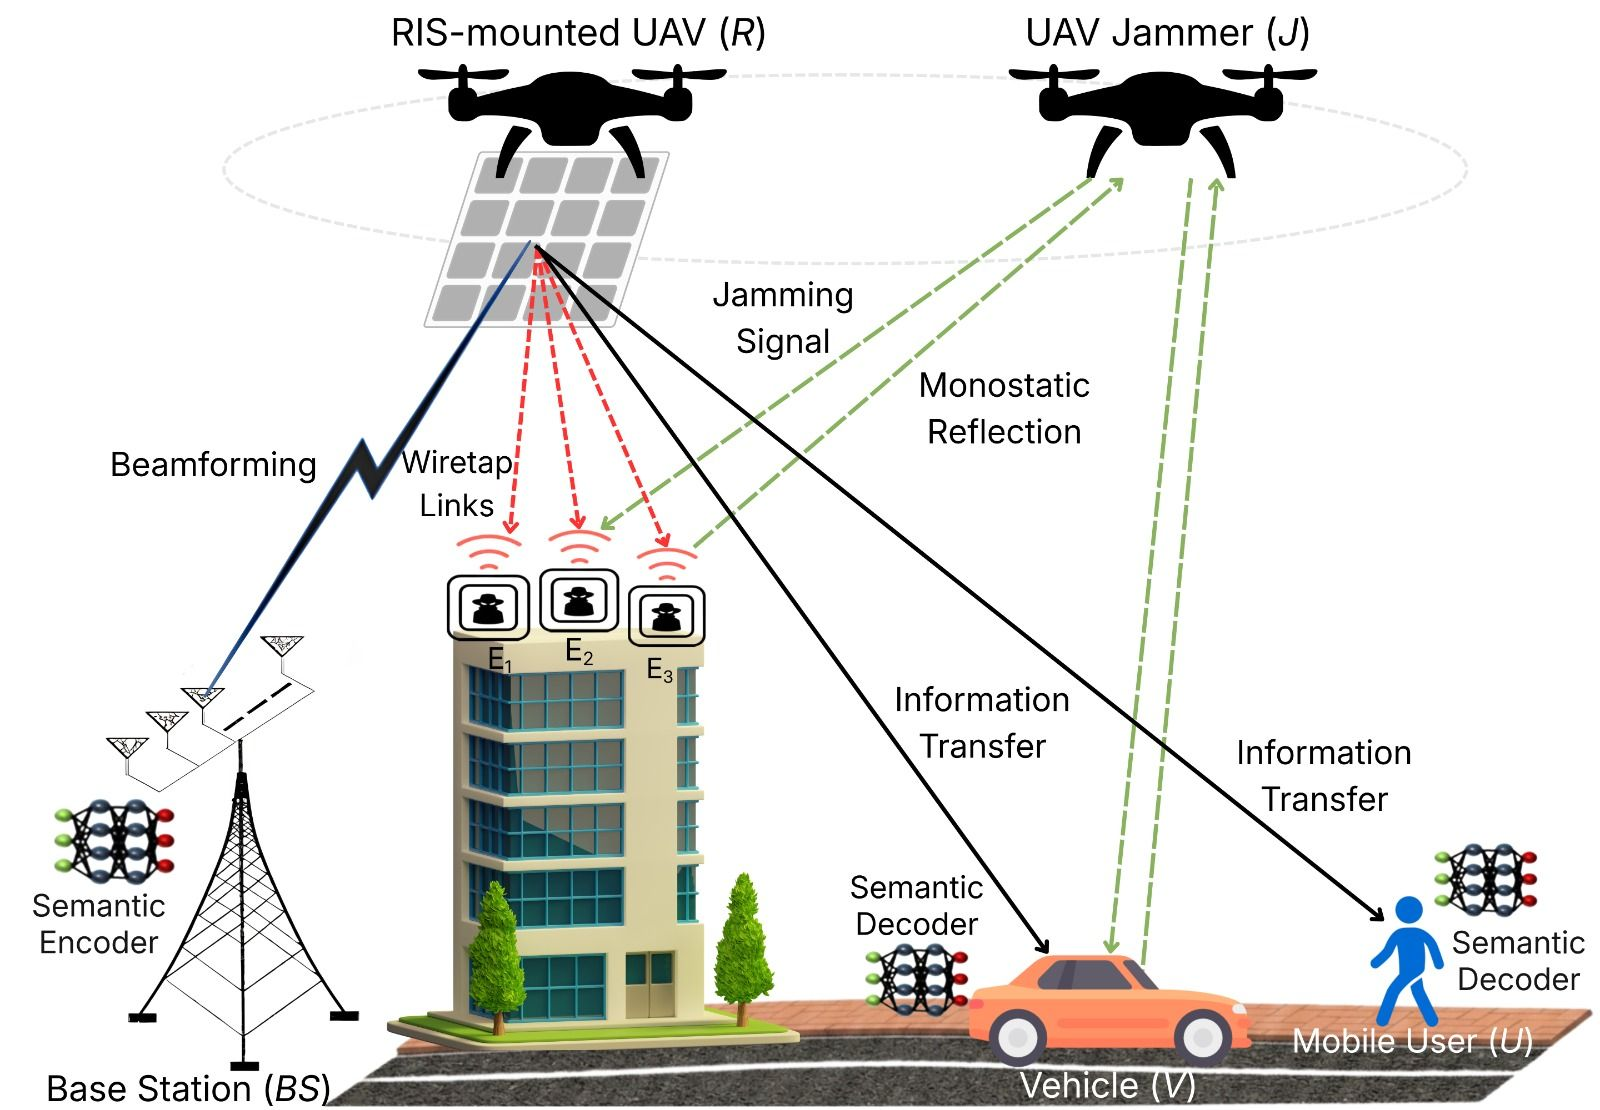
\includegraphics[width=0.65\textwidth]{system-model.jpeg}
    \caption{System model of the proposed semantic-aware RIS-assisted UAV ISAC network with friendly jamming and uncertain eavesdropper locations.}
    \label{fig:system_model}
\end{figure}

\section{System Architecture and Node Configuration}
We consider a 3D aerial-terrestrial network consisting of the following key nodes (see Fig.~\ref{fig:system_model}):
\begin{itemize}
    \item \textbf{Base Station ($B$)}: Located at $\mathbf{p}_B = [0, 0, 15]^T\text{ m}$, equipped with $N_B$ antennas, transmitting superposed PD-NOMA semantic signals with total power $P_B \in [0.5, 5.0]\text{ W}$ (nominal $2.0\text{ W}$).
    \item \textbf{RIS-mounted UAV ($R$)}: Hovering at $\mathbf{p}_R = [x_R, y_R, z_R]^T\text{ m}$ ($z_R \in [30, 100]\text{ m}$), equipped with $N_R = 64$ passive reflecting elements providing an array beamforming gain of $N_R^2 = 4096$.
    \item \textbf{UAV Jammer ($J$)}: An aerial platform hovering at $\mathbf{p}_J = [x_J, y_J, z_J]^T\text{ m}$ ($z_J \in [30, 100]\text{ m}$), transmitting artificial noise with power $P_J \in [0.05, 1.0]\text{ W}$ (nominal $0.5\text{ W}$) to jam eavesdroppers, while performing monostatic radar target tracking.
    \item \textbf{Target ($T$)}: A near legitimate vehicle located at $\mathbf{p}_T = [40, 45, 1.5]^T\text{ m}$. In the downlink, it decodes the NOMA superposed signal using semantic-aware SIC. In the uplink, it transmits messages to the BS via RIS and to the Mobile User $U$ via direct V2X with transmit power $P_T = 0.2\text{ W}$.
    \item \textbf{Mobile User ($U$)}: A far legitimate user located at $\mathbf{p}_U = [x_U, y_U, 1.5]^T\text{ m}$, undergoing random walk mobility with speed $v_U = 3.0\text{ m/s}$.
    \item \textbf{Eavesdroppers ($E_1, \dots, E_{K_e}$)}: Terrestrial non-colluding wiretap nodes located at uncertain positions with $K_e = 3$: $\widetilde{\mathbf{p}}_{E_1} = [70, 80, 0]^T$, $\widetilde{\mathbf{p}}_{E_2} = [90, 100, 0]^T$, and $\widetilde{\mathbf{p}}_{E_3} = [110, 110, 0]^T\text{ m}$.
\end{itemize}

\section{Mathematical Formulations}

\subsection{3D Elevation-Dependent Path Loss Model}
For any link between transmitter $i$ at $\mathbf{p}_i = [x_i, y_i, z_i]^T$ and receiver $j$ at $\mathbf{p}_j = [x_j, y_j, z_j]^T$, the 3D distance and 2D horizontal distance are:
\begin{equation}
    d_{ij} = \|\mathbf{p}_i - \mathbf{p}_j\|_2 = \sqrt{(x_i - x_j)^2 + (y_i - y_j)^2 + (z_i - z_j)^2}, \quad d_{\text{2D}, ij} = \sqrt{(x_i - x_j)^2 + (y_i - y_j)^2}.
\end{equation}
The elevation angle $\theta_{ij}$ (in degrees) is:
\begin{equation}
    \theta_{ij} = \arcsin\left( \frac{|z_i - z_j|}{d_{ij}} \right) \cdot \frac{180}{\pi}.
\end{equation}
The Line-of-Sight (LoS) probability is modeled via the environmental logistic function:
\begin{equation}
    P_{\text{LoS}}(\theta_{ij}) = \frac{1}{1 + a \cdot \exp\left( -b (\theta_{ij} - a) \right)}, \quad P_{\text{NLoS}}(\theta_{ij}) = 1 - P_{\text{LoS}}(\theta_{ij}),
\end{equation}
where $a = 9.61$ and $b = 0.16$ represent urban environment constants. The path loss expressions for LoS and NLoS states are:
\begin{equation}
    \text{PL}_{\text{LoS}}(d_{ij}) = 20\log_{10}\left( \frac{4\pi d_{ij} f_c}{c} \right) + \eta_{\text{LoS}}, \quad
    \text{PL}_{\text{NLoS}}(d_{ij}) = 20\log_{10}\left( \frac{4\pi d_{ij} f_c}{c} \right) + \eta_{\text{NLoS}},
\end{equation}
where $f_c = 2.4\text{ GHz}$, $c = 3 \times 10^8\text{ m/s}$, $\eta_{\text{LoS}} = 1.0\text{ dB}$, and $\eta_{\text{NLoS}} = 20.0\text{ dB}$. The average path loss in dB and linear scale is:
\begin{equation}
    \overline{\text{PL}}(d_{ij}, \theta_{ij}) = P_{\text{LoS}}(\theta_{ij}) \text{PL}_{\text{LoS}}(d_{ij}) + P_{\text{NLoS}}(\theta_{ij}) \text{PL}_{\text{NLoS}}(d_{ij}), \quad
    \text{PL}_{\text{linear}}(d_{ij}, \theta_{ij}) = 10^{-\overline{\text{PL}}(d_{ij}, \theta_{ij}) / 10}.
\end{equation}
Small-scale fading follows an elevation-dependent Rician distribution where the $K$-factor scales with $\theta_{ij}$:
\begin{equation}
    K_{\text{dB}}(\theta_{ij}) = K_0 + \alpha_K \theta_{ij} = 3.0 + 0.15 \theta_{ij}, \quad K(\theta_{ij}) = 10^{K_{\text{dB}}(\theta_{ij}) / 10},
\end{equation}
\begin{equation}
    g_{ij} = \text{PL}_{\text{linear}}(d_{ij}, \theta_{ij}) \cdot \left| \sqrt{\frac{K}{K+1}} \bar{\mathbf{h}}_{ij} + \sqrt{\frac{1}{K+1}} \tilde{\mathbf{h}}_{ij} \right|^2.
\end{equation}

\subsection{Multi-Stage Digital and Analog Beamforming}
\begin{enumerate}
    \item \textbf{Base Station Digital Beamforming}: The BS applies digital beamforming $\mathbf{w}_B \in \mathbb{C}^{N_B \times 1}$ ($\|\mathbf{w}_B\|_2 = 1$) to focus transmit energy toward the RIS UAV $R$.
    \item \textbf{RIS Analog Phase-Shift Beamforming}: The RIS phase-shift matrix is $\bm{\Phi} = \operatorname{diag}(e^{j\phi_1}, \dots, e^{j\phi_{N_R}})$. Coherent phase alignment yields a cascaded power gain scaling quadratically with $N_R$:
    \begin{equation}
        g_{\text{cascaded}, k} = g_{B,R} \cdot g_{R,k} \cdot N_R^2, \quad \forall k \in \{T, U\}.
    \end{equation}
    \item \textbf{Jammer Null-Space (NS) Beamforming}: The UAV Jammer projects artificial noise into the null space of legitimate channels ($\mathbf{h}_{J,T}$ and $\mathbf{h}_{J,U}$), achieving a spatial nulling rejection factor $\eta_{\text{ns}} = 10^{-4}$ ($-40\text{ dB}$ suppression) at legitimate nodes, while projecting full directional jamming onto eavesdroppers:
    \begin{equation}
        P_{J, k} = P_J \cdot g_{J,k} \cdot \eta_{\text{ns}}, \quad \forall k \in \{T, U, B\},
    \end{equation}
    \begin{equation}
        P_{J, E_e} = P_J \cdot g_{J, E_e}^{\min}, \quad \forall e \in \{1, \dots, K_e\}.
    \end{equation}
\end{enumerate}

\subsection{Power-Domain NOMA and Semantic SIC}
The BS superposes the Near user ($s_N$) and Far user ($s_F$) signals:
\begin{equation}
    s = \sqrt{a_N P_B} s_N + \sqrt{a_F P_B} s_F, \quad a_N + a_F = 1, \quad a_F > a_N \ge 0.
\end{equation}
\begin{itemize}
    \item \textbf{Far User (Mobile User $U$)} decodes $s_F$ treating $s_N$ as interference:
    \begin{equation}
        \gamma_F = \frac{a_F P_B g_U}{a_N P_B g_U + P_{J, U} + \sigma^2}.
    \end{equation}
    \item \textbf{Near User (Target $T$)} performs semantic SIC, decoding and subtracting $s_F$ before decoding $s_N$:
    \begin{equation}
        \gamma_N = \frac{a_N P_B g_T}{P_{J, T} + \sigma^2}.
    \end{equation}
\end{itemize}
Thermal noise power is set to $\sigma^2 = 10^{-13}\text{ W}$ ($-100\text{ dBm}$ for $B = 1\text{ MHz}$).

\subsection{Active Uplink and V2X Communication}
Target $T$ actively transmits with power $P_T = 0.2\text{ W}$:
\begin{itemize}
    \item \textbf{Uplink V2I (Target to BS via RIS)}: $\gamma_{\text{uplink}} = \frac{P_T g_{T, R, B}}{P_{J, B} + \sigma^2}$.
    \item \textbf{V2X Direct Semantic Link (Target to User $U$)}: $\gamma_{\text{V2X}} = \frac{P_T g_{T, U}}{P_{J, U} + \sigma^2}$.
\end{itemize}

\subsection{Monostatic and Bistatic Radar Sensing with Selection Combining}
To maximize radar coverage, the UAV Jammer performs selection combining between monostatic echo and bistatic BS-assisted sensing:
\begin{equation}
    \text{SNR}_{\text{radar}, T} = \max\left( \text{SNR}_{\text{mono}, T},\, \text{SNR}_{\text{bi}, T} \right), \quad
    \text{SNR}_{\text{radar}, E_e} = \max\left( \text{SNR}_{\text{mono}, E_e},\, \text{SNR}_{\text{bi}, E_e} \right),
\end{equation}
where:
\begin{equation}
    \text{SNR}_{\text{mono}, k} = \frac{P_{J} \cdot g_{J,k}^2 \cdot G_p}{\sigma^2}, \quad
    \text{SNR}_{\text{bi}, k} = \frac{P_B \cdot g_{B, k} \cdot g_{J, k} \cdot G_p}{\sigma^2}, \quad k \in \{T, E_e\},
\end{equation}
with radar processing gain $G_p = 10^4$. Detection probabilities follow empirical radar logistic curves:
\begin{equation}
    P_{d, k} = \frac{1}{1 + \exp\left( -\kappa (\text{SNR}_{\text{radar}, k, \text{dB}} - \tau) \right)}, \quad \kappa = 0.4, \ \tau = 2.0\text{ dB},
\end{equation}
\begin{equation}
    \text{CRB}_T = \frac{1}{\text{SNR}_{\text{radar}, T}}.
\end{equation}

\subsection{Worst-Case Eavesdropper Interception and Selection Combining Secrecy Rates}
Under bounded location uncertainty $\Delta Q_e = 15.0\text{ m}$, the worst-case eavesdropping channel minimizes 2D distance to the RIS and maximizes 2D distance to the Jammer:
\begin{equation}
    d_{\text{2D}, RE_e}^{\text{modified}} = \max(d_{\text{2D}, RE_e} - \Delta Q_e, 0), \quad
    d_{\text{2D}, JE_e}^{\text{modified}} = d_{\text{2D}, JE_e} + \Delta Q_e.
\end{equation}
The worst-case wiretap SINRs at eavesdropper $E_e$ are:
\begin{equation}
    \gamma_{E_e, U} = \frac{a_F P_B g_{E_e}^{\max}}{a_N P_B g_{E_e}^{\max} + P_J g_{J, E_e}^{\min} + \sigma^2}, \quad
    \gamma_{E_e, T} = \frac{a_N P_B g_{E_e}^{\max}}{P_J g_{J, E_e}^{\min} + \sigma^2}.
\end{equation}
For non-colluding eavesdroppers, the maximum interception rate across all $K_e$ eavesdroppers is evaluated:
\begin{equation}
    R_{\text{leak}, T} = \max_{e \in \{1, \dots, K_e\}} R_{\text{sem}, E_e, T}(\gamma_{E_e, T}), \quad
    R_{\text{leak}, U} = \max_{e \in \{1, \dots, K_e\}} R_{\text{sem}, E_e, U}(\gamma_{E_e, U}).
\end{equation}
The individual semantic secrecy rates for Target $T$ and Mobile User $U$ are:
\begin{equation}
    R_{\text{sec}, T} = \left[ R_{\text{sem}, T}(\gamma_N) - \max_{e \in \{1, \dots, K_e\}} R_{\text{sem}, E_e, T}(\gamma_{E_e, T}) \right]^+,
\end{equation}
\begin{equation}
    R_{\text{sec}, U} = \left[ R_{\text{sem}, U}(\gamma_F) - \max_{e \in \{1, \dots, K_e\}} R_{\text{sem}, E_e, U}(\gamma_{E_e, U}) \right]^+,
\end{equation}
where $[x]^+ = \max(x, 0)$. To combine communication security across both legitimate nodes, Selection Combining (SC) is applied:
\begin{equation}
    R_{\text{sec}}^{\text{SC}} = \max\left( R_{\text{sec}, T},\, R_{\text{sec}, U} \right), \quad R_{\text{sec}}^{\text{sum}} = R_{\text{sec}, T} + R_{\text{sec}, U}.
\end{equation}

\subsection{DeepSC Semantic Metric Formulation}
Semantic similarity $S(\gamma)$ is obtained via linear interpolation from Table~\ref{tab:deepsc_lookup}. With $M=10$ semantic concepts and $K=15$ channel symbols, the semantic rate (suts/s) and distortion are:
\begin{equation}
    R_{\text{sem}} = B \cdot \left( \frac{M}{K} \right) \cdot S(\gamma) \cdot \log_2(1 + \gamma), \quad D_{\text{sem}} = 1 - S(\gamma).
\end{equation}

\begin{table}[H]
    \centering
    \caption{DeepSC Lookup Table: SINR vs. Semantic Similarity and Word Accuracy ($M=10, K=15$).}
    \label{tab:deepsc_lookup}
    \begin{tabular}{ccc}
        \toprule
        $\gamma_{\text{dB}}$ (dB) & Semantic Similarity $S(\gamma)$ & Word Accuracy \\
        \midrule
        -20 & 0.6712 & 0.3945 \\
        -18 & 0.7171 & 0.4351 \\
        -16 & 0.7517 & 0.4549 \\
        -14 & 0.8021 & 0.4899 \\
        -12 & 0.8257 & 0.5261 \\
        -10 & 0.8638 & 0.5742 \\
        -8  & 0.8867 & 0.6012 \\
        -6  & 0.9103 & 0.6551 \\
        -4  & 0.9227 & 0.6830 \\
        -2  & 0.9316 & 0.6957 \\
        0   & 0.9398 & 0.7124 \\
        2   & 0.9443 & 0.7305 \\
        4   & 0.9456 & 0.7354 \\
        6   & 0.9462 & 0.7339 \\
        8   & 0.9490 & 0.7340 \\
        10  & 0.9499 & 0.7403 \\
        12  & 0.9504 & 0.7397 \\
        14  & 0.9508 & 0.7417 \\
        16  & 0.9508 & 0.7334 \\
        18  & 0.9508 & 0.7327 \\
        20  & 0.9507 & 0.7321 \\
        \bottomrule
    \end{tabular}
\end{table}

\begin{table}[H]
    \centering
    \caption{System Simulation and Channel Parameters.}
    \label{tab:system_params}
    \begin{tabular}{lcc}
        \toprule
        Parameter & Symbol & Value \\
        \midrule
        Carrier Frequency & $f_c$ & $2.4\text{ GHz}$ \\
        Channel Bandwidth & $B$ & $1.0\text{ MHz}$ \\
        Thermal Noise Power & $\sigma^2$ & $1.0 \times 10^{-13}\text{ W}$ ($-100\text{ dBm}$) \\
        BS Transmit Power Range & $P_B$ & $[0.5, 5.0]\text{ W}$ (Nominal: $2.0\text{ W}$) \\
        Jammer Transmit Power Range & $P_J$ & $[0.05, 1.0]\text{ W}$ (Nominal: $0.5\text{ W}$) \\
        Target Uplink Transmit Power & $P_T$ & $0.2\text{ W}$ ($23\text{ dBm}$) \\
        NOMA Far-User Allocation Range & $a_F$ & $[0.55, 0.95]$ (Nominal: $0.70$) \\
        Number of RIS Reflecting Elements & $N_R$ & $64$ ($N_R^2 = 4096$) \\
        Jammer Spatial Nulling Suppression & $\eta_{\text{ns}}$ & $1.0 \times 10^{-4}$ ($-40\text{ dB}$) \\
        Radar Processing Gain & $G_p$ & $1.0 \times 10^4$ ($40\text{ dB}$) \\
        Eavesdropper Uncertainty Radius & $\Delta Q_e$ & $15.0\text{ m}$ \\
        Number of Eavesdroppers & $K_e$ & $3$ \\
        DeepSC Concepts and Symbol Lengths & $M, K$ & $M=10, K=15$ ($M/K = 2/3$) \\
        CRB Feasibility Threshold & $\delta_{\text{CRB}}$ & $1.0 \times 10^8$ \\
        Radar Logistic Parameters & $\kappa, \tau$ & $\kappa = 0.4, \tau = 2.0\text{ dB}$ \\
        Urban LoS / NLoS Parameters & $a, b, \eta_{\text{LoS}}, \eta_{\text{NLoS}}$ & $9.61, 0.16, 1.0\text{ dB}, 20.0\text{ dB}$ \\
        \bottomrule
    \end{tabular}
\end{table}

\section{Multi-Objective Joint Secrecy and Sensing Optimization Problem}
The primary objective of the network is to jointly maximize communication secrecy and radar sensing performance under dynamic operational priorities. For an episode $e$ consisting of $T_{\text{total}}$ steps, the average secrecy rate under Selection Combining (SC) is:
\begin{equation}
    R_{\text{sec}}^{(e)} = \frac{1}{T_{\text{total}}} \sum_{t=1}^{T_{\text{total}}} R_{\text{sec}}^{\text{SC}}(t).
\end{equation}
The Average System Secrecy Ratio ($\operatorname{ASSR}^{(e)}$) is normalized to $[0, 1]$ via the running maximum reference $R_{\text{ref}}$:
\begin{equation}
    \operatorname{ASSR}^{(e)} = \operatorname{clip}\left( \frac{R_{\text{sec}}^{(e)}}{R_{\text{ref}}}, 0, 1 \right), \quad R_{\text{ref}} = \max_{j \in \{1, \dots, e\}} R_{\text{sec}}^{(j)}.
\end{equation}
The combined sensing detection probability is formulated as:
\begin{equation}
    P_d^{(e)} = \lambda_{1,\text{sense}} P_{d, E}^{(e)} + \lambda_{2,\text{sense}} P_{d, T}^{(e)}, \quad P_{d, E}^{(e)} = \frac{1}{K_e} \sum_{e=1}^{K_e} P_{d, E_e}^{(e)},
\end{equation}
where $\lambda_{1,\text{sense}}, \lambda_{2,\text{sense}} \ge 0$ ($\lambda_{1,\text{sense}} + \lambda_{2,\text{sense}} = 1$) are sensing priority weights (with nominal baseline $\lambda_{1,\text{sense}} = \lambda_{2,\text{sense}} = 0.5$).

Target tracking precision is strictly enforced via the CRB feasibility indicator:
\begin{equation}
    \mathbb{I}_{\text{CRB}}^{(e)} =
    \begin{cases}
        1, & \text{if } \operatorname{CRB}_{T}^{(e)} \le \delta_{\text{CRB}}, \\
        0, & \text{otherwise.}
    \end{cases}
\end{equation}

The unconstrained weighted multi-objective utility for episode $e$ is:
\begin{equation}
    \widehat{U}^{(e)} = \lambda_1 \operatorname{ASSR}^{(e)} + \lambda_2 P_d^{(e)},
\end{equation}
where $\lambda_1, \lambda_2 \ge 0$ ($\lambda_1 + \lambda_2 = 1$) are runtime user-configurable preference hyperparameters supplied at algorithm execution time to flexibly trade off between physical-layer semantic security and radar sensing detection capability.

The final constrained episode multi-objective utility is:
\begin{equation}
    U^{(e)} = \widehat{U}^{(e)} \cdot \mathbb{I}_{\text{CRB}}^{(e)} = \left( \lambda_1 \operatorname{ASSR}^{(e)} + \lambda_2 P_d^{(e)} \right) \mathbb{I}_{\text{CRB}}^{(e)}.
\end{equation}
In our comparative benchmark evaluation, we report results with the balanced operational trade-off $\lambda_1 = \lambda_2 = 0.5$.

\section{Deep Reinforcement Learning Algorithms and Formulations}
The decision process is modeled as an MDP $\langle \mathcal{S}, \mathcal{A}, \mathcal{P}, \mathcal{R}, \gamma \rangle$:
\begin{itemize}
    \item \textbf{State Space $\mathcal{S} \subset \mathbb{R}^{24}$}: Concatenation of 3D positions of all 8 nodes: $\mathbf{p}_B, \mathbf{p}_R, \mathbf{p}_J, \mathbf{p}_T, \mathbf{p}_U, \widetilde{\mathbf{p}}_{E_1}, \widetilde{\mathbf{p}}_{E_2}, \widetilde{\mathbf{p}}_{E_3}$.
    \item \textbf{Action Space $\mathcal{A} \subset \mathbb{R}^9$}: Partitioned into three sub-agents:
    \begin{itemize}
        \item Agent 1 (RIS UAV): $[\Delta x_R, \Delta y_R, \Delta z_R] \in [-5, +5]^3\text{ m}$.
        \item Agent 2 (Jammer UAV): $[\Delta x_J, \Delta y_J, \Delta z_J] \in [-5, +5]^3\text{ m}$.
        \item Agent 3 (Power Allocation): $[P_B, P_J, a_F] \in [0.5, 5.0]\text{ W} \times [0.05, 1.0]\text{ W} \times [0.55, 0.95]$.
    \end{itemize}
\end{itemize}

\subsection{Random Walk (Baseline)}
Actions are sampled uniformly at random: $a_{n,t} \sim \mathcal{U}(-1, 1)$.

\subsection{Single-Agent TD3PG (SATD3PG)}
A centralized actor network $\pi_\theta(s)$ controls all 9 action dimensions. The twin critics $Q_{\phi_1}, Q_{\phi_2}$ minimize:
\begin{equation}
    L(\phi_i) = \mathbb{E}\left[ \left( y_t - Q_{\phi_i}(s_t, a_t) \right)^2 \right], \quad
    y_t = r_t + \gamma \min_{j=1,2} Q_{\phi_j'}\left( s_{t+1}, \operatorname{clip}(\pi_{\theta'}(s_{t+1}) + \bm{\epsilon}, -1, 1) \right),
\end{equation}
with target policy smoothing $\bm{\epsilon} \sim \operatorname{clip}(\mathcal{N}(0, \sigma^2), -c, c)$ and delayed actor updates with frequency $d=2$:
\begin{equation}
    \nabla_\theta J(\theta) = \mathbb{E}\left[ \nabla_a Q_{\phi_1}(s, a)|_{a=\pi_\theta(s)} \nabla_\theta \pi_\theta(s) \right].
\end{equation}

\subsection{Single-Agent Soft Actor-Critic (SASAC)}
SASAC optimizes policy entropy alongside cumulative return:
\begin{equation}
    L(\phi_i) = \mathbb{E}\left[ \left( Q_{\phi_i}(s_t, a_t) - \left( r_t + \gamma \left( \min_{j=1,2} Q_{\phi_j'}(s_{t+1}, a_{t+1}) - \alpha_{\text{ent}} \log \pi_\theta(a_{t+1}|s_{t+1}) \right) \right) \right)^2 \right],
\end{equation}
\begin{equation}
    J(\theta) = \mathbb{E}\left[ \alpha_{\text{ent}} \log \pi_\theta(a_t|s_t) - \min_{j=1,2} Q_{\phi_j}(s_t, a_t) \right].
\end{equation}

\subsection{Multi-Agent TD3PG (MATD3PG)}
Three decentralized actor networks $\pi_{\theta_1}, \pi_{\theta_2}, \pi_{\theta_3}$ execute decentralized actions, while centralized twin critics $Q_{\phi_1}(s, a_1, a_2, a_3)$ evaluate joint actions:
\begin{equation}
    y_t = r_t + \gamma \min_{j=1,2} Q_{\phi_j'}\left( s_{t+1}, \pi_{\theta_1'}(s_{t+1}) + \bm{\epsilon}_1, \pi_{\theta_2'}(s_{t+1}) + \bm{\epsilon}_2, \pi_{\theta_3'}(s_{t+1}) + \bm{\epsilon}_3 \right),
\end{equation}
\begin{equation}
    \nabla_{\theta_n} J(\theta_n) = \mathbb{E}\left[ \nabla_{a_n} Q_{\phi_1}(s, a_1, a_2, a_3)|_{a_n=\pi_{\theta_n}(s)} \nabla_{\theta_n} \pi_{\theta_n}(s) \right].
\end{equation}

\subsection{Multi-Agent Proximal Policy Optimization (MAPPO)}
Three decentralized stochastic policy actors $\pi_{\theta_n}$ are trained with a centralized value function $V_\psi(s)$ using GAE ($\lambda_{\text{GAE}} = 0.95$):
\begin{equation}
    L^{\text{CLIP}}(\theta_n) = \mathbb{E}\left[ \min\left( \frac{\pi_{\theta_n}(a_{n,t}|s_t)}{\pi_{\theta_n}^{\text{old}}(a_{n,t}|s_t)} \widehat{A}_t, \operatorname{clip}\left( \frac{\pi_{\theta_n}(a_{n,t}|s_t)}{\pi_{\theta_n}^{\text{old}}(a_{n,t}|s_t)}, 1-\epsilon, 1+\epsilon \right) \widehat{A}_t \right) \right] + \beta_{\text{ent}} \mathcal{H}(\pi_{\theta_n}),
\end{equation}
\begin{equation}
    \widehat{A}_t = \sum_{l=0}^{T-t-1} (\gamma \lambda_{\text{GAE}})^l \delta_{t+l}^V, \quad \delta_t^V = r_t + \gamma V_\psi(s_{t+1}) - V_\psi(s_t), \quad
    L(\psi) = \mathbb{E}\left[ (V_\psi(s_t) - G_t)^2 \right].
\end{equation}

\begin{table}[H]
    \centering
    \caption{RL Training Hyperparameters.}
    \label{tab:hyperparameters}
    \begin{tabular}{lcccc}
        \toprule
        Hyperparameter & MAPPO & MATD3PG & SASAC & SATD3PG \\
        \midrule
        Number of Episodes & 8000 & 8000 & 8000 & 8000 \\
        Steps per Episode & 50 & 50 & 50 & 50 \\
        Batch Size & 64 & 64 & 64 & 64 \\
        Discount Factor $\gamma$ & 0.95 & 0.95 & 0.95 & 0.95 \\
        Soft Update $\tau$ & -- & 0.01 & 0.01 & 0.01 \\
        Replay Buffer Size & -- & 50000 & 50000 & 50000 \\
        Actor Learning Rate & $2.5 \times 10^{-4}$ & $3.0 \times 10^{-4}$ & $3.0 \times 10^{-4}$ & $3.0 \times 10^{-4}$ \\
        Critic Learning Rate & $2.5 \times 10^{-4}$ & $3.0 \times 10^{-4}$ & $3.0 \times 10^{-4}$ & $3.0 \times 10^{-4}$ \\
        Policy Noise $\sigma$ & -- & 0.2 & -- & 0.2 \\
        Noise Clip $c$ & -- & 0.5 & -- & 0.5 \\
        Policy Update Freq $d$ & -- & 2 & -- & 2 \\
        Entropy Coefficient $\beta_{\text{ent}} / \alpha_{\text{ent}}$ & 0.01 & -- & 0.2 & -- \\
        GAE Parameter $\lambda_{\text{GAE}}$ & 0.95 & -- & -- & -- \\
        PPO Clip Parameter $\epsilon$ & 0.2 & -- & -- & -- \\
        Gradient Clipping Norm & 0.5 & -- & -- & -- \\
        Hidden Layers & 2 (64 units) & 2 (64 units) & 2 (64 units) & 2 (64 units) \\
        Activation Function & ReLU & ReLU & ReLU & ReLU \\
        \bottomrule
    \end{tabular}
\end{table}

\begin{figure}[H]
    \centering
    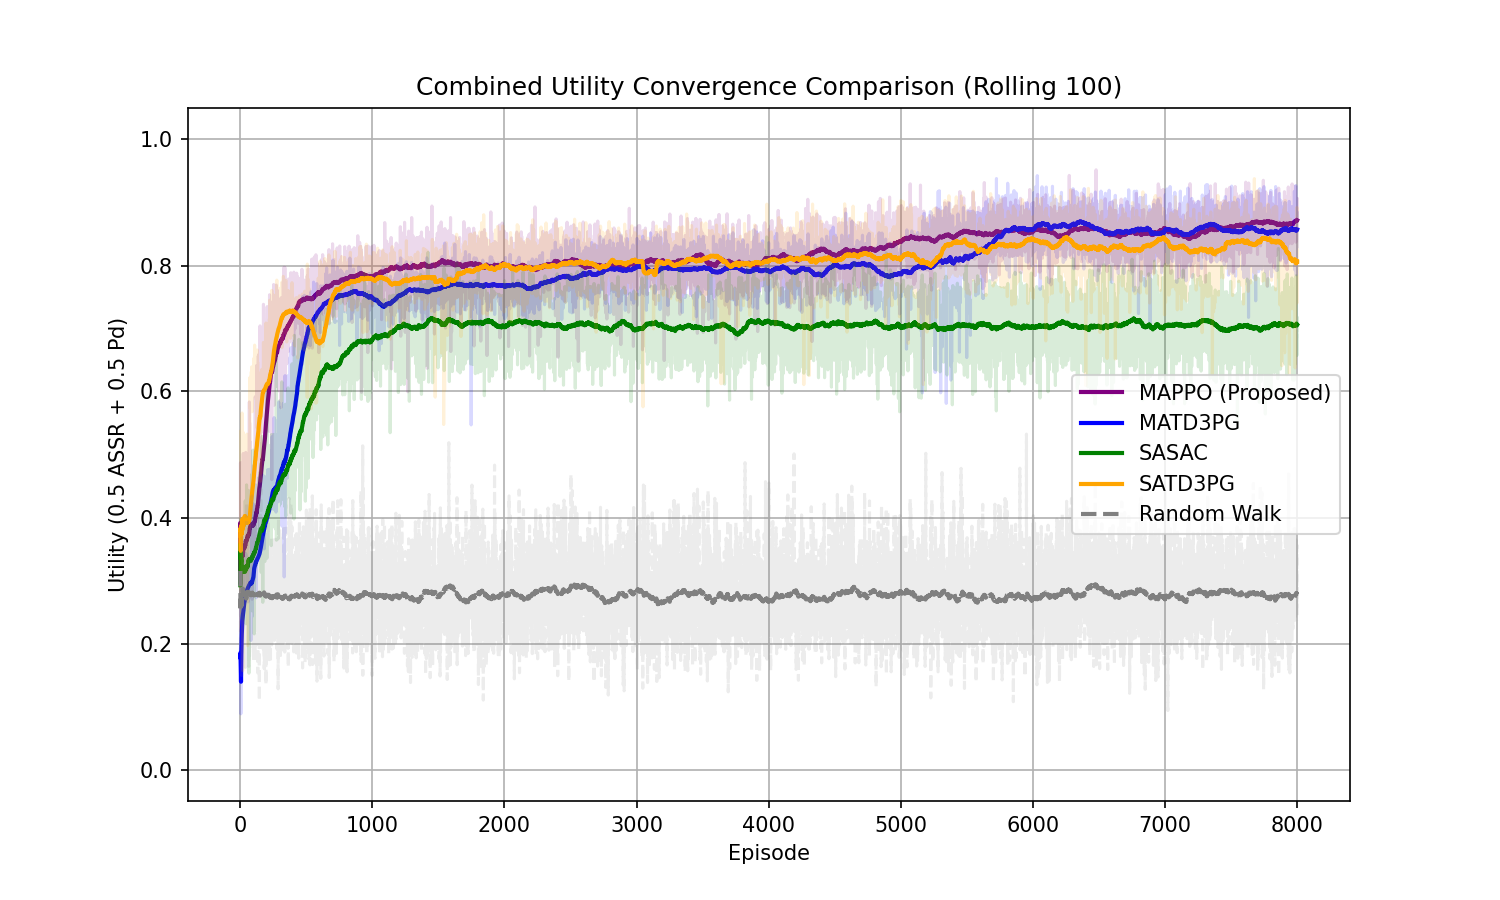
\includegraphics[width=0.68\textwidth]{convergence_comparison.png}
    \caption{Multi-objective utility convergence comparison ($U = \lambda_1\mathrm{ASSR} + \lambda_2 P_d$, benchmarked with $\lambda_1=\lambda_2=0.5$) across all five algorithms (MAPPO, MATD3PG, SASAC, SATD3PG, and Random Walk).}
    \label{fig:convergence}
\end{figure}

\begin{table}[H]
    \centering
    \caption{Convergence Performance Comparison under Location Uncertainty (Final Rolling-100 Benchmark).}
    \label{tab:convergence_results}
    \begin{tabular}{lcccc}
        \toprule
        Algorithm & Normalized ASSR & Detection Prob. ($P_d$) & Multi-Objective Utility ($U$) & Relative Rank \\
        \midrule
        \textbf{MAPPO (Proposed)} & \textbf{0.8418} & \textbf{0.9016} & \textbf{0.8717} & \textbf{1st (Best)} \\
        MATD3PG & 0.8134 & 0.9035 & 0.8585 & 2nd \\
        SATD3PG & 0.7644 & 0.8775 & 0.8210 & 3rd \\
        SASAC & 0.7089 & 0.7744 & 0.7416 & 4th \\
        Random Walk & 0.2312 & 0.4362 & 0.3337 & Baseline \\
        \bottomrule
    \end{tabular}
\end{table}

\section{Conclusion}
This report presented the comprehensive mathematical framework and empirical evaluation of a Semantic-Aware ISAC Network assisted by an aerial RIS and UAV Jammer under uncertain eavesdropper locations. By formulating multi-stage beamforming with friendly spatial nulling, Selection Combining across legitimate users and radar sensing branches, and DeepSC semantic lookup representations, the proposed architecture guarantees physical layer confidentiality and radar target tracking simultaneously. Reinforcement learning simulations demonstrate that the proposed decentralized Multi-Agent PPO (\textbf{MAPPO}) framework achieves superior convergence and stability, attaining the highest multi-objective utility of $\mathbf{0.8717}$ with an average normalized secrecy ratio of $\text{ASSR} = 0.8418$ and target detection probability exceeding $P_d = 0.9016$.

\bibliographystyle{IEEEtran}

\end{document}
